\chapter{Por qué la supersimetría podría ser importante}

\lectureoverview{Las fluctuaciones del vacío conectan los temas de este capítulo.
Las condiciones de contorno producen la fuerza de Casimir, los efectos de lazos ponen en riesgo la masa del Higgs, nuevas partículas virtuales modifican el comportamiento de los acoplamientos gauge con la escala y la energía del vacío gobierna la expansión cósmica. Estos problemas motivan la supersimetría a baja energía como una forma de estabilizar la escala del Higgs, proporcionar un candidato a materia oscura y mejorar la unificación de los acoplamientos gauge. Después construiremos supercampos usando coordenadas de Grassmann y emplearemos la integración de Berezin para obtener una acción supersimétrica.}

\section{Fluctuaciones del vacío entre placas reflectantes}

Retomamos la supersimetría resolviendo primero una cuestión sobre el efecto Casimir. Coloquemos dos placas reflectantes paralelas separadas una distancia \(d\). Aunque no haya partículas reales, un campo cuántico presenta fluctuaciones del vacío. Podemos imaginarlas como procesos virtuales o, de forma equivalente, como el movimiento de punto cero de los modos oscilatorios del campo. Las placas imponen condiciones de contorno, por lo que las fluctuaciones permitidas entre ellas difieren de las del espacio sin restricciones.

La magnitud importante no es un cero absoluto de energía, sino el cambio que se produce al variar la separación. Denotemos por \(\mathcal E(d)=E(d)/A\) la energía del vacío por unidad de área. Cuando \(\mathcal E\) depende de \(d\), se trata de una energía potencial, y la fuerza por unidad de área es
\begin{equation}
\frac{F}{A}=-\frac{d\mathcal E}{dd}.
\end{equation}
Así, una reorganización de los procesos virtuales se convierte en una fuerza observable. En el conocido ejemplo electromagnético con placas conductoras ideales, la energía y la presión son
\begin{align}
\mathcal E(d)&=-\frac{\pi^2}{720\,d^3},\\
\frac{F}{A}&=-\frac{\pi^2}{240\,d^4},
\end{align}
en unidades \(\hbar=c=1\).\editorialnote{Estos coeficientes y la distinción entre la energía por área \(d^{-3}\) y la presión \(d^{-4}\) resuelven la cuestión dimensional planteada en la pizarra. Son el resultado estándar para placas ideales; aquí no se deriva.} El signo menos indica atracción.

\begin{classroomqa}
\audiencequestion{¿La cuarta potencia describe la fuerza o la energía? \lecturetimestamp{00:04:39}}
\lecturerresponse{Para placas paralelas en cuatro dimensiones del espacio-tiempo, la energía por unidad de área disminuye como \(d^{-3}\), mientras que al derivar respecto de \(d\) la fuerza por unidad de área disminuye como \(d^{-4}\). El análisis dimensional ya determina estas potencias cuando se restituyen \(\hbar\) y \(c\).}
\end{classroomqa}

A veces se resume el cálculo diciendo que las placas interrumpen los lazos virtuales de fotones. Esa imagen es útil siempre que no se tome demasiado literalmente. El cálculo preciso consiste en un cambio del espectro de modos de campo permitidos o, de forma equivalente, un cambio de la acción efectiva cuántica. Ambos lenguajes conducen a la misma energía dependiente de la separación.

\begin{classroomqa}
\audiencequestion{¿Puede la fuerza de Casimir ser repulsiva en lugar de atractiva? \lecturetimestamp{00:07:48}}
\lecturerresponse{Sí. El signo no es universal: depende de los campos, la geometría, los materiales y las condiciones de contorno. Los lazos fermiónicos suelen aportar un signo de lazo opuesto al de los bosónicos, lo que motiva la sugerencia planteada en la pizarra; sin embargo, la estadística fermiónica por sí sola no constituye un teorema general según el cual toda fuerza de Casimir deba ser repulsiva.\editorialnote{Esta precisión sustituye una respuesta deliberadamente tentativa dada en clase por la afirmación general necesaria para evitar una regla universal falsa.}}
\end{classroomqa}

\subsection{¿Qué se consideraría evidencia de la energía del vacío?}

La fuerza de Casimir se mide, y los observables atómicos también son sensibles a los lazos del vacío. Sin embargo, ninguno de estos hechos demuestra por sí solo que la energía absoluta del vacío gravite. Un experimento de Casimir mide una diferencia de energía causada por las condiciones de contorno; es posible describir la misma fuerza sin atribuir significado operativo a una suma ilimitada de energías de punto cero absolutas.

La prueba decisiva viene de la gravedad. La energía es carga gravitatoria. Si el espacio vacío contiene una densidad de energía uniforme, esta debe aparecer en las ecuaciones de Einstein e influir en la expansión cósmica. Por tanto, la expansión acelerada del universo constituye la evidencia gravitatoria directa de un componente similar al vacío.

\begin{classroomqa}
\audiencequestion{¿Por qué los relatos divulgativos llaman misteriosa a la energía del vacío, como si los físicos no supieran qué es? \lecturetimestamp{00:08:19}}
\lecturerresponse{La teoría cuántica de campos asigna una contribución de punto cero a cada campo, así que la posibilidad de que exista energía del vacío no es misteriosa. El misterio es cuantitativo: ¿por qué el valor que gravita es extraordinariamente pequeño en comparación con las estimaciones basadas en los campos cuánticos conocidos y un corte de alta energía? Lo sorprendente es su casi total ausencia, no su mera presencia.}
\end{classroomqa}

Durante muchos años, el límite superior observacional era tan pequeño que resultaba psicológicamente tentador fijar la constante cosmológica exactamente en cero y buscar un principio que impusiera la cancelación. Las mejoras en las observaciones cosmológicas revelaron, en cambio, un valor pequeño pero distinto de cero. Ese descubrimiento no hizo que la energía del vacío resultara conceptualmente ajena; hizo imposible ignorar la magnitud de la supresión que aún no se explica. La comparación pertinente depende de la escala ultravioleta supuesta, pero toda estimación natural de alta energía exige una cancelación enorme.

\section{Qué hace una carga de supersimetría a un estado con muchas partículas}

Antes de enumerar razones para creer en la supersimetría, conviene despejar una posible paradoja. Los bosones pueden ocupar un mismo modo en cantidades arbitrariamente grandes, mientras que la ocupación de un modo fermiónico solo puede ser cero o uno. Si una simetría intercambia bosones y fermiones, ¿convierte mil bosones en un modo en mil fermiones prohibidos?

No. Un generador fermiónico cambia un cuanto cada vez. En el modelo de oscilador, sea \(a\) el operador que aniquila un bosón y \(c^\dagger\) el que crea su compañero fermiónico. Una carga de supersimetría puede representarse como
\begin{equation}
Q=c^\dagger a.
\end{equation}
Sobre un estado con \(n\) bosones y ningún fermión,
\begin{equation}
Q\ket{n,0}
=\sqrt n\,\ket{n-1,1}.
\end{equation}
Se ha eliminado un bosón y se ha insertado un fermión. Si se vuelve a aplicar la misma carga, el resultado es cero:
\begin{equation}
Q^2=(c^\dagger)^2a^2=0.
\end{equation}
Esta es la nilpotencia que se hereda de los operadores de creación fermiónicos.

\begin{classroomqa}
\audiencequestion{Si muchos bosones ocupan el mismo estado, ¿por qué una transformación de supersimetría no produce muchos fermiones en ese mismo estado y viola el principio de exclusión? \lecturetimestamp{00:12:05}}
\lecturerresponse{El generador no sustituye toda la población. Cambia el estado en una unidad de número fermiónico. La misma carga fermiónica no puede acumularse como un generador de rotaciones ordinario, porque su cuadrado se anula. Una carga complementaria puede deshacer el intercambio, y el anticonmutador mixto se cierra en una traslación temporal.}
\end{classroomqa}

La última frase es esencial. La forma abreviada \(Q^2=0\) se aplica a una componente quiral individual o a la carga sencilla que acabamos de escribir; no significa que se anule todo producto de cargas de supersimetría. En supersimetría en cuatro dimensiones,
\begin{equation}
\{Q_\alpha,\bar Q_{\dot\beta}\}
=2\sigma^\mu_{\alpha\dot\beta}P_\mu,
\end{equation}
mientras que
\begin{equation}
\{Q_\alpha,Q_\beta\}=0,
\qquad
\{\bar Q_{\dot\alpha},\bar Q_{\dot\beta}\}=0
\end{equation}
para el álgebra mínima sin cargas centrales.\editorialnote{Esta forma en componentes precisa la abreviatura usada en clase: la acción repetida de la misma carga de supersimetría \(Q\) se anula, mientras que una carga y su conjugada generan una traslación.}

\section{Tres razones para buscar supersimetría a baja energía}

\begin{classroomqa}
\audiencequestion{¿Hay motivos para la supersimetría además de cancelar la energía del vacío? \lecturetimestamp{00:15:06}}
\lecturerresponse{Hay tres motivos estrechamente relacionados: controlar la autoenergía del Higgs, contar con una posible partícula estable de materia oscura y lograr un encuentro mucho más preciso de los acoplamientos gauge a alta energía. Ninguno demuestra que la supersimetría se realice en la naturaleza, pero en conjunto hacen de ella una teoría seria que merece ponerse a prueba.}
\end{classroomqa}

La expresión \emph{supersimetría a baja energía} es relativa. No significa que los supercompañeros sean ligeros en la escala cotidiana, sino que sus masas no están muy por encima de las escalas electrodébil y de los aceleradores. Los tres argumentos se debilitan si las masas de los supercompañeros se elevan arbitrariamente.

\subsection{Proteger la escala del Higgs}

La masa de un escalar es excepcionalmente sensible a la física de alta energía. Esquemáticamente, un lazo bosónico produce una corrección de la forma
\begin{equation}
\delta m_H^2\big|_{\mathrm B}
\sim +\frac{\lambda}{16\pi^2}\Lambda^2,
\end{equation}
donde \(\Lambda\) representa la escala hasta la que se utiliza la teoría efectiva. Un lazo fermiónico lleva el signo opuesto,
\begin{equation}
\delta m_H^2\big|_{\mathrm F}
\sim -\frac{|y|^2}{8\pi^2}\Lambda^2.
\end{equation}
Los coeficientes dependen de la interacción y de las multiplicidades de los campos, pero la supersimetría los relaciona de tal modo que la sensibilidad ultravioleta dominante se cancela entre los supercompañeros.\editorialnote{Las fórmulas esquemáticas de los lazos muestran la matemática que subyace al argumento cualitativo sobre la autoenergía. No pretenden ser un cálculo completo de la masa del Higgs del Modelo Estándar.}

Esto importa porque el valor esperado del Higgs fija la escala electrodébil. Las masas de los bosones gauge y de los fermiones obedecen relaciones como
\begin{equation}
m_W=\frac{gv}{2},
\qquad
m_f=\frac{y_fv}{\sqrt2}.
\end{equation}
Si el sector del Higgs tendiera de forma natural a una escala enorme, se perdería el espectro de partículas conocido a baja energía, a menos que se ajustaran los parámetros desnudos contra las correcciones radiativas con una precisión extrema.

La supersimetría exacta haría exacta la cancelación, pero ya está descartada por las masas desiguales de los bosones y fermiones observados. Con supersimetría rota suavemente, la sensibilidad cuadrática se sustituye por una dependencia de las diferencias de masa entre supercompañeros, esquemáticamente
\begin{equation}
\delta m_H^2
\sim
\frac{g^2}{16\pi^2}
\left(m_{\mathrm{soft}}^2-m_{\mathrm{ordinary}}^2\right)
\ln\frac{\Lambda^2}{m_{\mathrm{soft}}^2}.
\end{equation}
La cancelación solo resulta útil mientras la diferencia de masas no sea demasiado grande.

\subsection{Un estado final estable para las cascadas de materia oscura}

Dividamos el espectro entre partículas ordinarias y sus supercompañeros. Un fermión tiene un supercompañero bosónico; un bosón, uno fermiónico. Si las interacciones conservan una paridad que distingue estas dos clases, la desintegración de un supercompañero debe dejar otro supercompañero:
\begin{equation}
\widetilde X
\longrightarrow X+\widetilde Y
\longrightarrow X+Y+\widetilde Z
\longrightarrow\cdots.
\end{equation}
La cascada no puede descartar su último supercompañero. Por tanto, termina en la partícula supersimétrica más ligera, el LSP.

La simetría que se usa habitualmente es la paridad \(R\),
\begin{equation}
R_p=(-1)^{3(B-L)+2s}.
\end{equation}
Las partículas del Modelo Estándar tienen \(R_p=+1\), mientras que sus supercompañeros tienen \(R_p=-1\). Si \(R_p\) es exacta, toda interacción contiene un número par de supercompañeros y el LSP es estable.\editorialnote{La supersimetría por sí sola no garantiza que el LSP sea estable. La estabilidad requiere que se conserve la paridad \(R\) u otra simetría con la misma consecuencia; sin ella, el LSP puede desintegrarse.}

La materia oscura debe sobrevivir al menos durante escalas de tiempo cosmológicas. También debe interactuar con suficiente debilidad como para atravesar repetidamente el disco galáctico visible sin perder una cantidad sustancial de energía. Una población con carga eléctrica o interacciones fuertes dispersaría, disiparía energía y tendería a colapsar hasta formar la misma estructura delgada que la materia ordinaria. El halo extendido observado apunta, en cambio, a un componente neutro y débilmente interactuante.

Esto no identifica de manera única al LSP. Según el modelo y el patrón de ruptura de la simetría, el candidato podría ser una mezcla neutra de gauginos electrodébiles e higgsinos, o bien un gravitino. Los candidatos cargados o coloreados están fuertemente restringidos. Lo que aporta la supersimetría no es una respuesta garantizada, sino un mecanismo natural para producir un estado final neutro y longevo.

\section{Acoplamientos variables con la escala y el indicio de unificación}

El tercer motivo parte del apantallamiento de la carga. Un acoplamiento medido depende de la escala de energía porque las partículas virtuales modifican la interacción. En el electromagnetismo, un lazo electrón-positrón insertado en un propagador del fotón apantalla la carga a larga distancia. A distancias menores, o con mayor transferencia de momento, queda menos nube de polarización entre las partículas de prueba y la carga efectiva es mayor.

Escribamos
\begin{equation}
\alpha_i=\frac{g_i^2}{4\pi}.
\end{equation}
A un lazo, el inverso del acoplamiento varía linealmente con el logaritmo de la energía:
\begin{equation}
\frac{d\alpha_i^{-1}}{d\ln\mu}
=-\frac{b_i}{2\pi}.
\end{equation}
Así,
\begin{equation}
\alpha_i^{-1}(\mu)
=\alpha_i^{-1}(\mu_0)
-\frac{b_i}{2\pi}\ln\frac{\mu}{\mu_0}.
\end{equation}
\editorialnote{Esta ecuación a un lazo es la formulación precisa de las rectas casi perfectas que se dibujan en función del logaritmo de la energía. Los umbrales y las correcciones de órdenes superiores curvan ligeramente las líneas.}

Por encima de la escala electrodébil, los tres acoplamientos gauge fundamentales corresponden a
\begin{equation}
U(1)_Y,\qquad SU(2)_L,\qquad SU(3)_c.
\end{equation}
El acoplamiento electromagnético que se emplea para orientarse a baja energía es una combinación de los dos primeros tras la ruptura de la simetría electrodébil. En QCD, los campos gauge no abelianos producen antiapantallamiento: el acoplamiento fuerte disminuye a distancias cortas, fenómeno conocido como libertad asintótica. Por consiguiente, \(\alpha_3^{-1}\) aumenta con \(\ln\mu\), mientras que los inversos de los otros acoplamientos tienen pendientes distintas.

Las curvas del Modelo Estándar apuntan sugestivamente unas hacia otras, pero no se cruzan en un único punto. Los supercompañeros modifican los lazos virtuales y, por tanto, cambian los coeficientes \(b_i\). En la normalización convencional de gran unificación,
\begin{align}
(b_1,b_2,b_3)_{\mathrm{SM}}
&=\left(\frac{41}{10},-\frac{19}{6},-7\right),\\
(b_1,b_2,b_3)_{\mathrm{MSSM}}
&=\left(\frac{33}{5},1,-3\right).
\end{align}
Con umbrales de los supercompañeros cerca de la escala del TeV, las curvas supersimétricas extrapoladas se encuentran con mucha más precisión cerca de
\begin{equation}
M_{\mathrm{GUT}}\sim 10^{16}\ \mathrm{GeV}.
\end{equation}
Ningún experimento alcanza directamente esa escala. Se miden los acoplamientos a baja energía, el contenido de campos determina su evolución con la escala y las curvas se extrapolan a lo largo de muchas décadas. Dos líneas siempre se cruzan en algún punto; que tres líneas independientes se encuentren cerca de un mismo punto es la observación no trivial.

\begin{classroomqa}
\audiencequestion{¿La extrapolación mejorada supone supersimetría exacta y masas iguales para los supercompañeros? \lecturetimestamp{00:38:09}}
\lecturerresponse{No. La supersimetría está rota, así que las masas son distintas. Lo que importa es cuándo empiezan a contribuir los lazos de los supercompañeros a la evolución de los acoplamientos. Si no son demasiado pesados, las pendientes cambian con suficiente antelación para que converjan los tres acoplamientos. Si son extremadamente pesados, los umbrales supersimétricos aparecen demasiado tarde y se pierde el encuentro más preciso.}
\end{classroomqa}

Las correcciones de umbral y el espectro desconocido de alta energía impiden afirmar literalmente que las tres líneas se encuentran con exactitud matemática. Aun así, el resultado es sorprendente: la misma escala aproximada de los supercompañeros que ayuda con el Higgs y proporciona un candidato a materia oscura térmica también mejora la unificación.

\subsection{La gravedad y la escala común de alta energía}

La gravedad se comporta de otra manera porque su carga es la propia energía. Una medida adimensional útil a una energía del centro de masas \(E\) es
\begin{equation}
\alpha_G(E)\sim GE^2
=\left(\frac{E}{M_{\mathrm{Pl}}}\right)^2.
\end{equation}
A energías ordinarias es extraordinariamente pequeña, pero crece cuadráticamente con \(E\). Por eso, su inversa disminuye mucho más rápido que los inversos de los acoplamientos gauge, que varían logarítmicamente, y se vuelve del orden de la unidad cerca de la escala de Planck.

Esta comparación sugiere que todas las interacciones podrían estar regidas por escalas altas cercanas entre sí, pero es menos clara que la unificación gauge. Los acoplamientos gauge son parámetros adimensionales en teorías de campos renormalizables; la constante de Newton tiene dimensiones, por lo que representar la gravedad en la misma gráfica requiere adoptar una convención.

\begin{classroomqa}
\audiencequestion{¿Los supercompañeros participan en las mismas tres interacciones gauge o definen fuerzas nuevas? \lecturetimestamp{00:42:35}}
\lecturerresponse{Tienen los mismos números cuánticos gauge que sus compañeros. Un selectrón tiene la carga eléctrica del electrón, y un escuark tiene el color y las cargas electrodébiles correspondientes a las del quark, aunque sus espines y masas sean distintos. Por tanto, sus lazos modifican las mismas interacciones gauge, en lugar de introducir tres interacciones nuevas.}
\end{classroomqa}

\begin{classroomqa}
\audiencequestion{¿El descubrimiento de un supercompañero en el LHC sería una prueba definitiva de la supersimetría? \lecturetimestamp{00:43:27}}
\lecturerresponse{Una sola partícula desconocida no bastaría por el mero hecho de llevar ese nombre, pero un espectro de supercompañeros que obedeciera las relaciones supersimétricas entre espines, cargas, masas y acoplamientos sería muy distintivo. La supersimetría impone muchas restricciones correlacionadas, por lo que el patrón detallado de interacciones proporcionaría la prueba decisiva.}
\end{classroomqa}

\subsection{Por qué no se puede desplazar la escala sin pagar un precio}

Si los supercompañeros están apenas más allá del alcance experimental, los tres motivos aún pueden ser válidos. Si sus masas aumentan varios órdenes de magnitud, cada argumento pierde fuerza:
\begin{enumerate}\item Las cancelaciones de la masa del Higgs dejan una gran sensibilidad residual a la diferencia de masas.
\item Ya no aparece una reliquia térmica convencional de escala electrodébil en la escala esperada.
\item Los umbrales de la evolución de los acoplamientos se desplazan hacia arriba y los tres acoplamientos se encuentran con menor precisión.
\end{enumerate}
La supersimetría aún podría existir a una escala mucho mayor, pero ya no resolvería estos problemas concretos de baja energía con la misma economía. La longevidad de la idea no demuestra que la naturaleza tenga que emplearla; demuestra que la propuesta es coherente y merece una prueba decisiva.

\section{Qué puede y qué no puede decirnos la cosmología sobre la materia oscura}

\begin{classroomqa}
\audiencequestion{¿Puede la cosmología estándar determinar la cantidad de materia oscura y la masa de cada partícula de materia oscura, del mismo modo que la nucleosíntesis permite restringir las cantidades de hidrógeno y helio? \lecturetimestamp{00:46:32}}
\lecturerresponse{La cosmología mide muy bien la densidad total de masa de materia oscura, pero la densidad por sí sola no permite separar la masa del número de partículas. La misma densidad podría corresponder a unas pocas partículas pesadas o a un número enorme de partículas muy ligeras. Para identificar la partícula microscópica hace falta teoría adicional u observaciones no gravitatorias.}
\end{classroomqa}

Dos posibilidades generales ilustran esta ambigüedad. Una partícula débilmente interactuante, cercana a la escala electrodébil o del TeV, puede desacoplarse térmicamente de un baño caliente. En el extremo opuesto, un bosón extremadamente ligero, como el axión, puede ocupar una configuración de campo coherente o un condensado. Las posibilidades intermedias no quedan descartadas solo porque los dos mecanismos mejor desarrollados se encuentren cerca de extremos opuestos.

La propia estructura del halo impone una restricción importante. La materia oscura atraviesa la materia ordinaria con poca fricción, por lo que permanece extendida espacialmente en lugar de colapsar en el disco luminoso. Las curvas de rotación y otros fenómenos gravitatorios nos indican que la masa está presente, pero no permiten contar las partículas por sí solos.

\begin{classroomqa}
\audiencequestion{¿Es posible que el universo primitivo contuviera inicialmente solo superpartículas, que luego se desintegraran en las partículas que observamos? \lecturetimestamp{00:49:11}}
\lecturerresponse{A temperaturas mucho mayores que todas las masas pertinentes, las reacciones rápidas llevan las especies al equilibrio térmico, en lugar de mantener una población unilateral arbitraria. Las colisiones ordinarias crean supercompañeros cuando estos escasean, mientras que las colisiones y desintegraciones de supercompañeros reponen las partículas ordinarias. La abundancia precisa depende de las interacciones y de los grados de libertad, pero el plasma caliente tiende continuamente al equilibrio.}
\end{classroomqa}

A medida que el universo se enfría, las especies masivas quedan suprimidas por el factor de Boltzmann y se aniquilan o desintegran. Un LSP estable deja de seguir el equilibrio cuando su tasa de interacción se vuelve más lenta que la expansión cósmica:
\begin{equation}
\Gamma_{\mathrm{ann}}
\sim n\langle\sigma v\rangle
\lesssim H.
\end{equation}
Las partículas restantes constituyen una abundancia relicta.\editorialnote{Este criterio de desacoplamiento completa de forma cuantitativa el argumento del equilibrio térmico. Otros candidatos a LSP, en especial los gravitinos con acoplamiento muy débil, pueden tener historias no térmicas.}

\begin{classroomqa}
\audiencequestion{¿De qué partícula ordinaria es supercompañero el LSP, y debe carecer de interacciones? \lecturetimestamp{00:51:05}}
\lecturerresponse{No hay una respuesta independiente del modelo. Se espera que un LSP viable como materia oscura sea eléctricamente neutro y no tenga color, pero no tiene por qué carecer por completo de interacciones. Puede ser una mezcla relacionada con el fotón, los bosones gauge débiles y los campos del Higgs, o puede ser el gravitino. Su identidad precisa se deduce del espectro de ruptura de la supersimetría.}
\end{classroomqa}

\section{Diagramas del vacío, diagramas de autoenergía y expansión}

\begin{classroomqa}
\audiencequestion{¿Cuál es la diferencia entre la divergencia del Higgs y la divergencia de la energía del vacío? \lecturetimestamp{00:52:09}}
\lecturerresponse{Un diagrama del vacío no tiene líneas externas de partículas; modifica la acción efectiva del espacio vacío y contribuye a la energía del vacío. Un diagrama de autoenergía del Higgs tiene dos líneas externas del Higgs; modifica el propagador del Higgs y, por tanto, su masa. Ambos implican fluctuaciones virtuales, pero responden a preguntas distintas.}
\end{classroomqa}

Podemos imaginar una partícula real como una impureza insertada en el vacío. Las fluctuaciones del vacío que se acoplan a ella modifican su propagación y su masa. Las placas de Casimir también modifican las fluctuaciones del vacío, pero mediante condiciones de contorno macroscópicas. En todos los casos, el elemento común es la respuesta de las fluctuaciones cuánticas a algo que se ha introducido; lo que difiere es el observable cuya corrección se calcula.

\vspace{-2pt}
\subsection{La materia, la radiación y el vacío se diluyen de maneras distintas}

Sea \(a(t)\) el factor de escala cosmológico y
\begin{equation}
H=\frac{\dot a}{a}
\end{equation}
el parámetro de Hubble. La conservación local del tensor de energía-momento en un universo homogéneo da
\begin{equation}
\dot\rho+3H(\rho+p)=0.
\end{equation}
Para una ecuación de estado \(p=w\rho\), esto se integra y da
\begin{equation}
\rho(a)\propto a^{-3(1+w)}.
\end{equation}
\editorialnote{La ecuación de continuidad proporciona la derivación concisa que sustenta las explicaciones basadas en el recuento de partículas y el estiramiento de las longitudes de onda.}

Para la materia fría no relativista, \(p\approx0\), así que
\begin{equation}
\rho_m\propto a^{-3}.
\end{equation}
Un volumen comóvil fijo crece como \(a^3\), mientras que la energía en reposo transportada por sus partículas permanece aproximadamente constante.

Para la radiación, \(p=\rho/3\), y
\begin{equation}
\rho_r\propto a^{-4}.
\end{equation}
Tres potencias proceden de la dilución de la densidad numérica. La cuarta se debe al corrimiento al rojo:
\begin{equation}
\lambda\propto a,
\qquad
E_\gamma=\frac{2\pi\hbar c}{\lambda}\propto a^{-1}.
\end{equation}

\begin{classroomqa}
\audiencequestion{Si un fotón tiene una función de onda, ¿por qué podemos hablar de él como partícula y no como onda al derivar la ley de dilución? \lecturetimestamp{00:58:21}}
\lecturerresponse{La distinción no afecta a la dependencia con la escala. En la descripción de partículas, el número de cuantos en un volumen comóvil permanece fijo y cada cuanto experimenta un corrimiento al rojo como \(a^{-1}\). En la descripción de ondas clásicas, la longitud de onda se estira y la energía del campo disminuye en la misma proporción. Podemos usar el lenguaje que haga más fácil visualizar la expansión.}
\end{classroomqa}

La energía del vacío tiene \(p_\Lambda=-\rho_\Lambda\), así que
\begin{equation}
\rho_\Lambda=\text{constant}.
\end{equation}
No se diluye al expandirse el espacio. De hecho, una región comóvil contiene
\begin{equation}
E_\Lambda=\rho_\Lambda a^3V_0,
\end{equation}
que crece con su volumen físico. Este hecho plantea la cuestión de la conservación de la energía que abordaremos en breve.

Las distintas potencias organizan la historia cósmica. La radiación disminuye más deprisa, la materia disminuye más lentamente y la energía del vacío no disminuye en absoluto. Por tanto, un término de vacío diminuto puede ser insignificante en el universo temprano y dominar en épocas tardías. Según los valores aproximados comentados aquí, el presupuesto energético actual consta de aproximadamente \(70\%\) de energía del vacío y \(30\%\) de materia, con una contribución de radiación mucho menor.

\section{La geometría es igual a la energía}

La componente tiempo-tiempo de las ecuaciones de Einstein convierte las leyes de escala anteriores en dinámica. La pizarra empieza con un lema y un único término geométrico.

\begin{figure}[H]
\centering
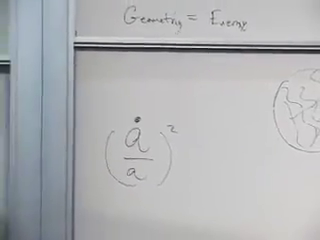
\includegraphics[width=0.68\textwidth]{lecture_06_figure_03.png}
\lectureframe{01:06:37.088}
\caption{El lema organizador \emph{la geometría es igual a la energía}, con el término de expansión \(H^2=(\dot a/a)^2\) escrito debajo.}
\end{figure}

Para un universo homogéneo e isótropo, la primera ecuación de Friedmann es
\begin{equation}
H^2+\frac{k}{a^2}
=\frac{8\pi G}{3}\rho,
\end{equation}
en unidades \(c=1\), donde \(k=+1,0,-1\) denota una geometría espacial cerrada, plana o abierta, y
\begin{equation}
\rho
=\rho_{\mathrm{ordinary}}
+\rho_{\mathrm{dark}}
+\rho_{\mathrm{radiation}}
+\rho_{\mathrm{vacuum}}.
\end{equation}
El signo que aparece junto a \(1/a^2\) depende de si el término de curvatura se deja a la izquierda o se pasa a la derecha, así como del valor de \(k\).

\begin{figure}[H]
\centering
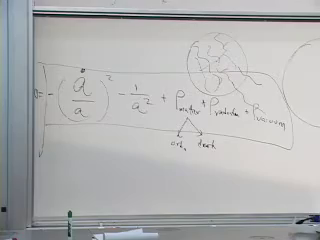
\includegraphics[width=0.96\textwidth]{lecture_06_figure_04.png}
\lectureframe{01:08:46.794}
\caption{El balance completo de la pizarra: expansión y curvatura espacial en el lado geométrico, y materia, radiación y energía del vacío en el lado de las fuentes. La materia se desglosa además en componentes ordinaria y oscura.}
\end{figure}

\subsection{La restricción hamiltoniana cosmológica}

\begin{classroomqa}
\audiencequestion{Si la energía del vacío en una región comóvil crece al expandirse el universo, ¿hay una densidad de energía neta constante o una energía total conservada? \lecturetimestamp{01:01:51}}
\lecturerresponse{La relatividad general no proporciona una energía global universal para un espacio-tiempo expansivo arbitrario. Sin embargo, en la reducción cosmológica homogénea, la ecuación de Einstein tiempo-tiempo es una restricción hamiltoniana. Cuando se colocan la geometría y la materia en un mismo lado, el hamiltoniano restringido se anula. Los términos de materia variables quedan compensados por los grados de libertad gravitatorios, y no por una energía ordinaria fija dentro de una caja.}
\end{classroomqa}

Esquemáticamente, la formulación canónica es
\begin{equation}
\mathcal H_{\mathrm{gravity}}
+\mathcal H_{\mathrm{matter}}
=0.
\end{equation}
Este es el significado preciso de afirmar que la energía total es cero. Se trata de una ecuación de movimiento impuesta por la invariancia ante reparametrizaciones temporales, no de afirmar que toda densidad de energía local se anule. En un volumen comóvil, la energía de la materia ordinaria se mantiene aproximadamente constante, la energía de la radiación disminuye y la energía del vacío aumenta; mientras tanto, la contribución gravitatoria y la tasa de expansión se ajustan para que la restricción de Einstein siga satisfaciéndose.

La conservación local sigue siendo exacta:
\begin{equation}
\nabla_\mu T^{\mu\nu}=0.
\end{equation}
Para el fluido homogéneo, esta es precisamente la ecuación de continuidad
\(\dot\rho+3H(\rho+p)=0\). Lo que en general deja de cumplirse es la intuición propia del espacio-tiempo plano de que también debe existir una única suma global de la energía de la materia, independiente de las coordenadas, que se conserve en un universo en expansión.\editorialnote{Esta distinción precisa la afirmación didáctica de que la energía siempre es cero: la conservación covariante local y la restricción hamiltoniana cosmológica son exactas, mientras que, en general, no está definida una energía global única de materia más gravedad.}

\begin{classroomqa}
\audiencequestion{¿Es la restricción de energía nula la condición que determina si el universo es abierto, cerrado o plano? \lecturetimestamp{01:04:42}}
\lecturerresponse{No. La restricción hamiltoniana se aplica en todos los casos. Los universos abiertos, planos y cerrados se distinguen por el parámetro de curvatura \(k\) y, por tanto, por el término \(k/a^2\). La curvatura modifica una contribución al balance; no activa ni desactiva la restricción.}
\end{classroomqa}

\section{Coordenadas de Grassmann y supercampos}

\begin{classroomqa}
\audiencequestion{¿Aparecen realmente los números de Grassmann en el lagrangiano de la teoría? \lecturetimestamp{01:09:37}}
\lecturerresponse{Aparecen primero porque los campos fermiónicos son impares de Grassmann. Aparecen una segunda vez como coordenadas del espacio supersimétrico. Los supercampos dependen de esas coordenadas impares, y las acciones supersimétricas se construyen derivando e integrando con respecto a ellas.}
\end{classroomqa}

Un campo ordinario es una función del espacio-tiempo,
\begin{equation}
\phi=\phi(x^\mu).
\end{equation}
La supersimetría mínima en cuatro dimensiones amplía \(x^\mu\) con un espinor impar de dos componentes \(\theta^\alpha\) y su conjugado \(\bar\theta^{\dot\alpha}\):
\begin{equation}
z^M=(x^\mu,\theta^\alpha,\bar\theta^{\dot\alpha}).
\end{equation}
Hay dos componentes impares complejas, o cuatro direcciones impares reales. Un supercampo es una función definida en este espacio supersimétrico:
\begin{equation}
\Phi=\Phi(x,\theta,\bar\theta).
\end{equation}

Estas no son dimensiones espaciales diminutas en el sentido métrico. Una coordenada de Grassmann no tiene una magnitud numérica positiva. Llamarla pequeña es una regla mnemotécnica para recordar la nilpotencia:
\begin{equation}
(\theta^\alpha)^2=0,
\qquad
\theta^\alpha\theta^\beta=-\theta^\beta\theta^\alpha.
\end{equation}
\editorialnote{La razón por la que toda expansión en un número finito de coordenadas de Grassmann termina es la nilpotencia, no la pequeñez numérica.}

Con cuatro coordenadas impares independientes, un supercampo completamente general tiene como máximo \(2^4=16\) monomios de Grassmann. Esquemáticamente,
\begin{equation}
\begin{aligned}
\Phi(x,\Theta)={}&\phi(x)+\Theta_A\psi_A(x)\\
&+\frac{1}{2}\Theta_A\Theta_B Z_{AB}(x)+\cdots\\
&+\Theta_1\Theta_2\Theta_3\Theta_4D(x),
\end{aligned}
\end{equation}
donde \(\Theta_A\) representa colectivamente las cuatro coordenadas impares reales. Como se puede elegir que el supercampo completo sea par, los coeficientes de las potencias pares son bosónicos y los de las potencias impares son fermiónicos. Así, un supercampo reúne un multiplete finito de campos componentes ordinarios.

Esta forma de agruparlos es más que una notación. La supersimetría actúa geométricamente como una traslación en las direcciones impares, combinada con una traslación en el espacio-tiempo. Un lagrangiano construido a partir de supercampos según las reglas del espacio supersimétrico hereda la simetría, del mismo modo que un lagrangiano escalar construido a partir de tensores hereda la invariancia rotacional o de Lorentz.

La acción incluye ahora medidas de Grassmann. Un término típico de espacio supersimétrico completo tiene la forma
\begin{equation}
S_D=\int d^4x\,d^2\theta\,d^2\bar\theta\,
\mathcal K(\Phi,\Phi^\dagger).
\end{equation}
Los términos quirales usan, en cambio,
\begin{equation}
S_F=\int d^4x\,d^2\theta\,W(\Phi)+\mathrm{h.c.}
\end{equation}
\editorialnote{La distinción entre medidas de espacio supersimétrico completo y medidas quirales es el refinamiento estándar de la acción esquemática \(d^4x\,d^4\theta\). Los ejemplos concretos determinarán qué medida corresponde utilizar.}

Hemos llegado, por tanto, a una pregunta que el cálculo ordinario no responde: ¿qué significa integrar respecto de una coordenada anticonmutativa?

\section{Integración de Berezin}

\subsection{El modelo ordinario: una derivada total}

Comencemos con una función ordinaria \(F(x)\) que se anula cuando \(x\) tiende a valores positivos y negativos grandes. El teorema fundamental del cálculo da
\begin{equation}
\int_{-\infty}^{\infty}dx\,\frac{dF}{dx}
=F(\infty)-F(-\infty)
=0.
\end{equation}

\begin{figure}[H]
\centering
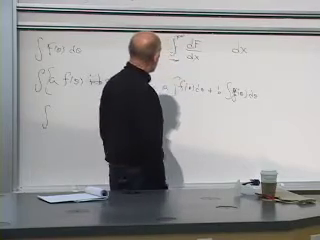
\includegraphics[width=0.88\textwidth]{lecture_06_figure_05.png}
\lectureframe{01:26:31.594}
\caption{El modelo ordinario de la integración de Berezin: la integral de una derivada total se reduce a los valores en los extremos y se anula cuando la función tiende a cero. La línea inferior de la pizarra está parcialmente tapada, así que el texto presenta la ecuación sin obstrucciones.}
\end{figure}

Queremos que la integral de Grassmann sea lineal y comparta la propiedad útil de que la integral de una derivada total se anule. Para una coordenada impar, exigimos
\begin{align}
\int d\theta\,[af(\theta)+bg(\theta)]
&=
a\int d\theta\,f(\theta)
+b\int d\theta\,g(\theta),\\
\int d\theta\,\partial_\theta f(\theta)&=0.
\end{align}
La segunda condición es el análogo algebraico de la invariancia de la medida ante traslaciones. No hay extremos de una recta numérica impar ni una suma sobre intervalos diminutos.

\begin{classroomqa}
\audiencequestion{Si no existe una integral indefinida de Grassmann, ¿estamos abandonando la idea de que integrar es la operación inversa de derivar? \lecturetimestamp{01:21:19}}
\lecturerresponse{Sí. La integración de Berezin es un funcional lineal definido, no una operación de hallar primitivas. De hecho, para una variable de Grassmann, está representada por la misma operación algebraica que la derivación.}
\end{classroomqa}

\begin{classroomqa}
\audiencequestion{¿La integración respecto de \(d^4x\) todo el espacio-tiempo también es una integral definida? \lecturetimestamp{01:21:34}}
\lecturerresponse{Sí. Al integrar la acción sobre el espacio-tiempo se sobreentienden las condiciones de contorno. La diferencia es que la integración ordinaria sobre el espacio-tiempo puede entenderse mediante límites de sumas, mientras que la integración de Grassmann se define algebraicamente por su acción sobre la base finita \(1,\theta\).}
\end{classroomqa}

\subsection{Una variable}

Toda función de una variable impar se puede escribir con su coeficiente en el orden fijo, a la derecha:
\begin{equation}
f(\theta)=a+\theta b.
\end{equation}
Como \(\partial_\theta\theta=1\), la regla para las derivadas totales implica
\begin{equation}
\int d\theta\,1=0.
\end{equation}
La normalización restante se elige como
\begin{equation}
\int d\theta\,\theta=1.
\end{equation}
Por consiguiente,
\begin{equation}
\int d\theta\,f(\theta)=b.
\end{equation}
La integral selecciona el coeficiente de la potencia más alta disponible. Con la convención de derivada por la izquierda usada aquí,
\begin{equation}
\partial_\theta f=b
=\int d\theta\,f.
\end{equation}

\begin{classroomqa}
\audiencequestion{¿Existe una función \(F(\theta)\) que satisfaga \(\partial_\theta F=\theta\)? \lecturetimestamp{01:30:05}}
\lecturerresponse{No. Tal función tendría que incluir un término proporcional a \(\theta^2\), pero \(\theta^2=0\). Esta es otra manera de ver por qué no existe un análogo de una primitiva indefinida para las variables de Grassmann.}
\end{classroomqa}

\subsection{Dos variables y el orden de la medida}

Para un par complejo \(\theta,\bar\theta\), escribamos una función general par en la forma ordenada
\begin{equation}
f(\theta,\bar\theta)
=a+\bar\theta\psi+\bar\psi\theta+b\,\bar\theta\theta.
\end{equation}
No hay términos de orden superior porque
\begin{equation}
\theta^2=\bar\theta^2=0,
\qquad
\bar\theta\theta=-\theta\bar\theta.
\end{equation}

Fijamos ahora la convención
\begin{equation}
\int d\theta\,d\bar\theta\,
\bar\theta\theta=1.
\end{equation}
En las integrales iteradas, la operación adyacente \(d\bar\theta\) actúa primero. La tabla queda entonces
\begin{align}
\int d\theta\,d\bar\theta\,1&=0,\\
\int d\theta\,d\bar\theta\,\theta&=0,\\
\int d\theta\,d\bar\theta\,\bar\theta&=0,\\
\int d\theta\,d\bar\theta\,\bar\theta\theta&=1.
\end{align}
Por tanto,
\begin{equation}
\int d\theta\,d\bar\theta\,
f(\theta,\bar\theta)=b.
\end{equation}

\begin{classroomqa}
\audiencequestion{Para un término lineal en \(\theta\), ¿es realmente la integración respecto de \(\theta\) la que hace que la integral doble se anule? \lecturetimestamp{01:34:59}}
\lecturerresponse{No; la explicación oral invirtió los papeles. Integrar \(\theta\) con respecto a \(\theta\) da uno. El resultado ya no contiene \(\bar\theta\), y la integral restante de uno respecto de \(\bar\theta\) se anula. En cualquier caso, la integral doble solo es distinta de cero cuando aparecen ambas variables.}
\end{classroomqa}

\begin{classroomqa}
\audiencequestion{Si se intercambian \(\theta\) y \(\bar\theta\), ¿cambia de signo la integral? \lecturetimestamp{01:36:33}}
\lecturerresponse{Sí. Las variables impares y las medidas impares anticonmutan. Con la convención anterior,
\[
\int d\bar\theta\,d\theta\,\bar\theta\theta=-1.
\]
Por tanto, hay que elegir un orden y mantenerlo de manera coherente. La física es independiente de la convención, pero los signos intermedios no lo son.}
\end{classroomqa}

Para \(n\) variables de Grassmann independientes, el patrón es inmediato:
\begin{equation}
\int d\theta_n\cdots d\theta_1\,
f(\theta_1,\ldots,\theta_n)
\end{equation}
extrae el coeficiente del monomio de grado máximo ordenado
\(\theta_1\cdots\theta_n\), con el signo determinado por el orden elegido para las variables y las medidas. Esta sencilla regla de extracción de componentes es la clave de las acciones en el espacio supersimétrico. Una variación supersimétrica se convierte en una derivada total impar, y la integral en el espacio supersimétrico la elimina, del mismo modo que una acción ordinaria elimina una derivada total en el espacio-tiempo bajo condiciones de contorno adecuadas.

\section{Por qué un cálculo tan sencillo tiene tanta potencia}

Las reglas parecen casi triviales:
\begin{equation}
\int d\theta\,1=0,
\qquad
\int d\theta\,\theta=1.
\end{equation}
Sin embargo, nos permiten construir teorías de campos con interacciones en las que las relaciones entre las masas y los acoplamientos bosónicos y fermiónicos se conservan automáticamente. El propósito del cálculo en el espacio supersimétrico es el mismo que el del cálculo tensorial en relatividad: organizar la notación de modo que la simetría deseada se conserve en todas las manipulaciones permitidas.

Llevar la cuenta de los signos es el precio. Cada intercambio de dos objetos impares aporta un signo menos, y un cálculo puede ser conceptualmente correcto y, aun así, fallar por una elección equivocada del orden. Esta dificultad no es decorativa: es la manifestación algebraica de la estadística fermiónica.

\begin{classroomqa}
\audiencequestion{¿Se inventaron los números de Grassmann junto con la supersimetría o ya existían antes? \lecturetimestamp{01:41:19}}
\lecturerresponse{Son mucho más antiguos. Hermann Grassmann desarrolló el álgebra exterior subyacente en el siglo XIX. Las formas diferenciales ya usan elementos de base anticonmutativos; la teoría cuántica de campos y la supersimetría del siglo XX encontraron un nuevo papel físico para las mismas matemáticas.}
\end{classroomqa}

Ya estamos preparados para realizar construcciones concretas. Los supercampos reúnen multipletes completos de bosones y fermiones, las derivadas en el espacio supersimétrico preservan el álgebra y la integración de Berezin extrae la acción en términos de componentes. La tarea siguiente consiste en emplear estas herramientas en el modelo unidimensional más sencillo y luego extenderlas a la teoría de campos.
